\section{Simulation} \label{sec:sim}

In this section, Monte Carlo (MC) simulations of the performance and characteristics of machined scintillators are discussed.  These studies were performed using the GEANT4 tool-kit which simulates the passage of particles through matter \cite{geant4_website}.  Comparisons are made with data observed in experiments conducted on the bench in Sec.~\ref{sec:fab_test} and with beam data in Sec.~\ref{sec:perform}.  

% WB I would merge the full simulation and the simplified one as they do not need to be considered separately
% show results for the unified model only
% EP reduced the amount of detail in the simple and unified sections

\subsection{Simulating a Simplified Model of the ST} \label{sec:sim_simple}

As discussed in Sec.~\ref{sec:design_paddles}, the ST scintillator paddles have a unique geometry in which the nose section tapers in width as the paddles approach the beam line at the downstream end.  This tapering effect results in a unique phenomenon in which the light output of the scintillator paddle begins to increase as the source moves further away from the readout detector.  This phenomenon is completely contrary to what one might expect. In the traditional sense when the source moves further away from the end being readout, the photons have a larger effective path length and thus, have an increased probability in being lost for detection.  However, this is antithetical relative to what is observed on the bench and in Hall-D.

A simple GEANT4 simulation was conducted to investigate the aforementioned phenomenon. The details of the simulation are discussed in Ref.~\cite{pooser16}.  Only the two trapezoidal regions of a machined scintillator paddle were considered.  Namely, the wide straight section and the tapered nose section. % which are illustrated in the GEANT4 event display seen in Fig. \ref{fig:100_events}.
%	\begin{figure}[!htb]
%	\centering
%	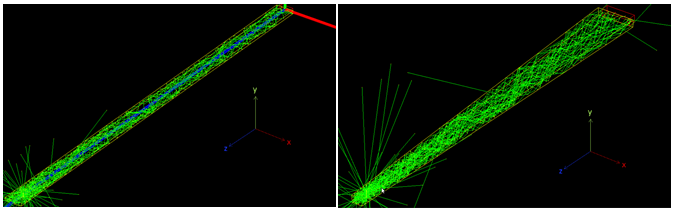
\includegraphics[width=1.0\columnwidth]{simulation/figs/100_events}
%	\caption{100 Optical photons generated in the staight \& nose sections.  Left: wide straight section.  Right: tapered nose section.  The neon green lines are the paths of the optical photons.  It is clear that some photons do in fact escape the scintillator medium, while others are collected in the simulated SiPM detector.}
%	\label{fig:100_events}
%	\end{figure}
% WB this plot can be skipped
% EP done.
%	\begin{figure}[!htb]
%	\centering
%	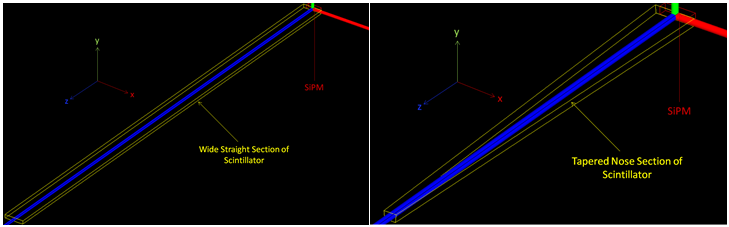
\includegraphics[width=1.0\columnwidth]{simulation/figs/beam_off}
%	\caption{Simulated straight \& nose section geometries.  Shown is the GEANT4 event display.  Left: wide straight section.  Right: tapered nose section.  The sections have been oriented such that they are in the same coordinate system as defined in HallD.  The yellow lines are the scintillator boundaries, while the red lines are the boundaries of the SiPM.}
%	\label{fig:beam_off}
%	\end{figure}  

%The EJ-200 scintillator material ($\rho=1.023~\mathrm{g/cc^{3}}$, $n = 1.58$) \cite{ej200_specs} was simulated with only one free parameter utilized to characterize the scintillator bar \textit{i.e.}, the reflectivity of the \textit{G4LogicalSkinSurface}, was set to 98\% so there remained some finite probability that photons could be lost in the scintillator medium.  Furthermore, the SiPM readout detector was placed at the upstream end of the two sections, seen in Fig. \ref{fig:100_events}.  Moreover, the SiPM was constructed as a \textit{G4SensitiveDetector} made of Silicon with a 100\% detection efficiency.  The SiPM was constructed to have an active area of $\mathrm{3 \times 12~mm^2}$ which is identical to the readout system described in Sec.~\ref{sec:design_sipms}.

%The EJ-200 scintillator material was simulated with only one free parameter in order to characterize the properties of the scintillator geometry.  The reflectivity of the boundaries was configured to be 98\% so that there existed a finite probability that photons could be lost at the scintillator boundaries.  The SiPM readout detector was configured with 100\% detection efficiency and constructed with the same active area as was discussed in Sec.~\ref{sec:design_sipms}.  The SiPM detector was placed at the upstream end of the two sections, seen in Fig. \ref{fig:100_events}.

%In order to simulate a charged particle traversing through the scintillator medium resulting in the production of photons along its path through the material, optical photons were generated inside the volume of the simulated scintillator material.  The scintillation yield was defined to be $\mathrm{10,000~ \gamma 's / 1~MeV}$ \cite{ej200_specs}.  For visual purposes, Fig. \ref{fig:100_events} shows 100 optical photons being produced at the tip of the downstream end of the two sections of the simulated scintillator paddle.

In order to sample the entirety of the two sections, 10,000 optical photons were generated at 16 different locations inside the medium of the scintillator. 
% WB this plot can be skipped
% EP done.
%	\begin{figure}[!htb]
%	\centering
%	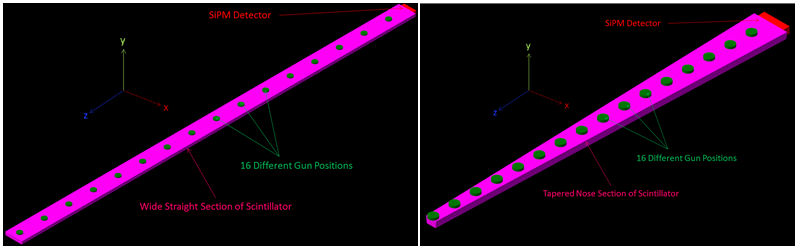
\includegraphics[width=1.0\columnwidth]{simulation/figs/gun_locations}
%	\caption{Optical photon gun locations along the straight \& nose sections. Left: wide straight section.  Right: tapered nose section.  The magenta geometries indicate the scintillator boundaries of the two sections.  The red box is the sensitive SiPM detector, and the green cylinders represent the location of the 16 optical photon gun locations. The locations of the source were chosen to be equal distances apart relative to each of the two sections.}
%	\label{fig:gun_locations}
%	\end{figure}
The photon energies ranged between $0.5 - 3.0$ eV \cite{krane_ch7} and were generated randomly in $4\pi$ along a 3 mm path $(y-axis)$ in the scintillator medium.  The path was oriented orthogonal to the wide surface of the scintillator.  
%In essence, this simulates a charged particle traversing through the medium with a $\theta_{track} = 90^{\circ}$ in hall coordinates.  
The number of photons collected by the SiPM at each of the source locations was counted and correlated to the source location.  The results can be seen in Fig. \ref{fig:sim_results}.
% WB this plot can be skipped
% EP keeping this plot here so that the simple results are illustrated
	\begin{figure}[!htb]
	\centering
	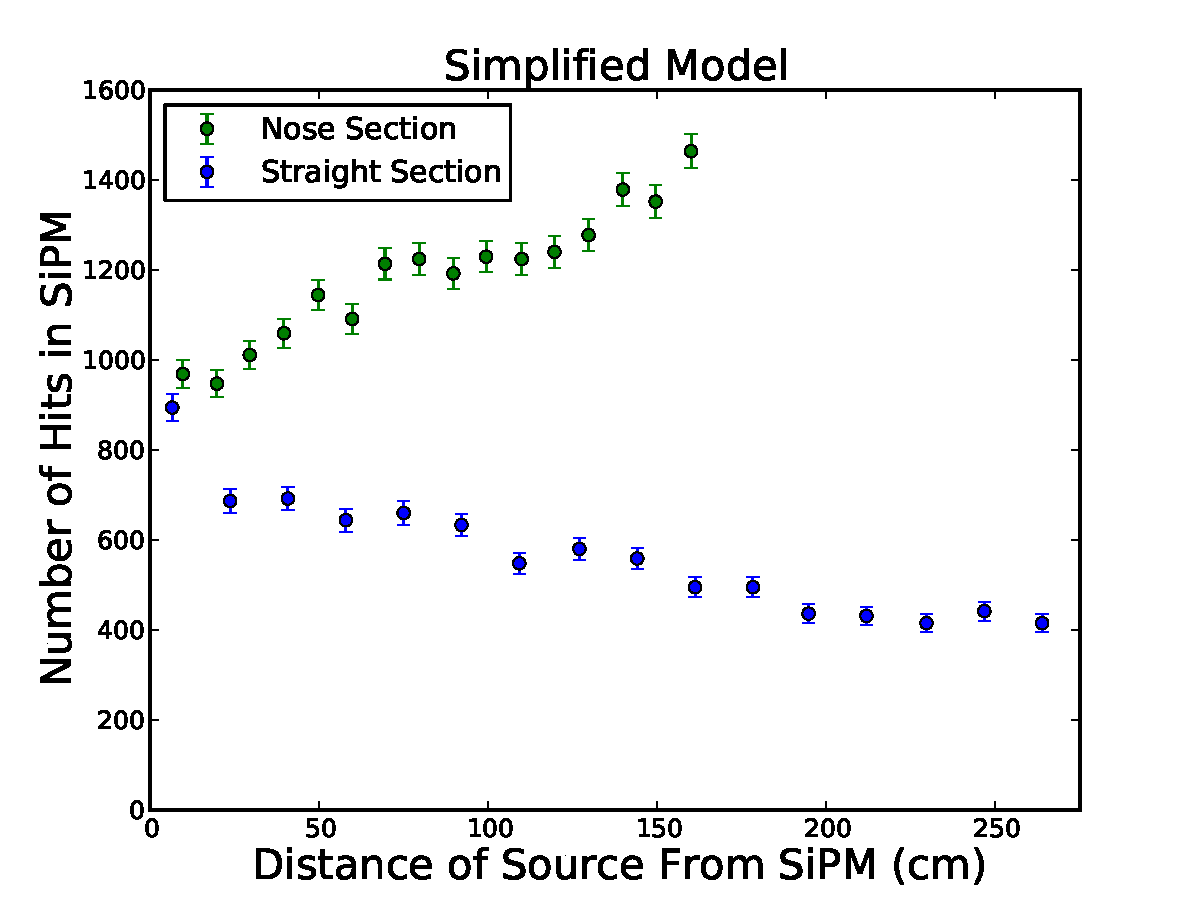
\includegraphics[width=1.0\columnwidth]{simulation/figs/sim_results_v4}
	\caption{Simulation results for simplified two section scenario. The total number of photons which were collected by the SiPM detector at each of the 16 source locations is plotted against the source distance from the sensitive detector.}
	\label{fig:sim_results}
	\end{figure}

From the data it is clear that the geometry of the nose section results in an improvement of light collection as the source moves further away from the readout detector.  In fact, there is a factor $\approx 1/2$ light loss observed in the straight section upon comparing the number of hits collected at the closest and furthest locations relative to the readout detector.  However, there is factor $\approx 3/2$ light gain observed in the nose region.

These results are primarily due to the tapering trapezoidal geometry in the nose section.  This phenomenon is not observed in the quasi-rectangular straight section as it exhibits a more conventional behavior. However, this behavior in the nose region is advantageous since the majority of forward going charged particles will traverse through the this region.

\subsection{Simulating Machined Scintillator Geometry} \label{sec:sim_mach}

Further studies were conducted to simulate more realistically the effects of light collection that results from the ST scintillator geometry and optical surface quality.  The ST scintillator geometry was imported into GEANT4 from a Vectorworks CAD drawing utilizing the CADMesh utility \cite{cadmesh_g4} and is shown \textit{via} the GEANT4 event display in Fig. \ref{fig:pk_cadmesh}.
% WB this figure needs to be bigger, 3d is enough
% EP removed top view and added picture with 100 optical photons
	\begin{figure}[!htb]
	\centering
	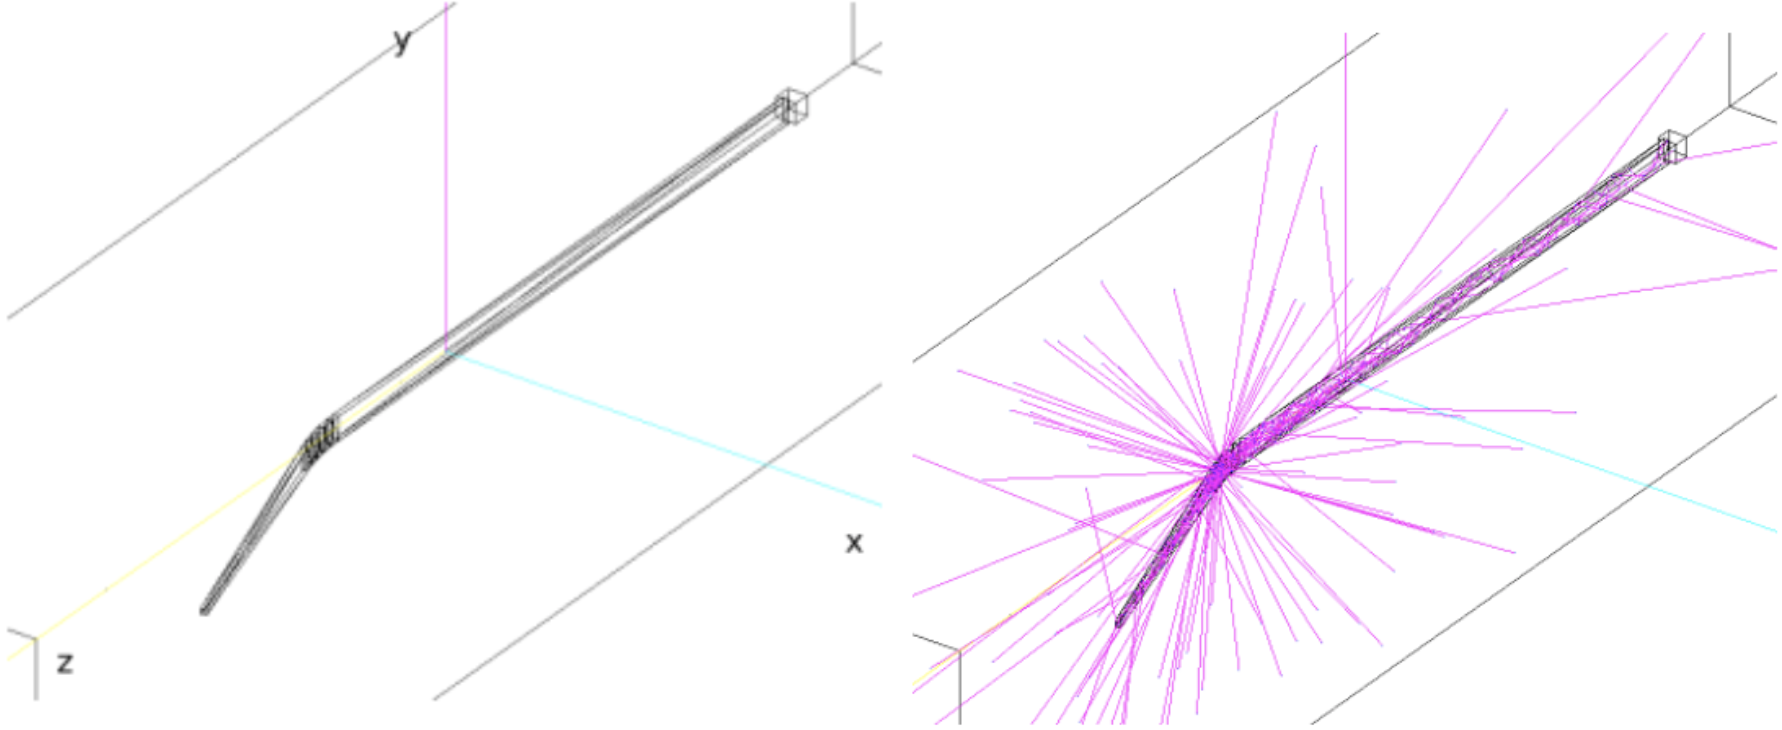
\includegraphics[width=1.0\columnwidth]{simulation/figs/pk_cadmesh_v2}
	\caption{Scintillator geometry imported into GEANT4 utilizing the CADMesh Utility.  The scintillator is  coupled to a SiPM detector.  Left: isometric view.  Right: isometric view with 100 optical photons being generated in the middle of the bend section.  The tapering of the nose section is clearly visible.}
	\label{fig:pk_cadmesh}
	\end{figure}
The SiPM was constructed as a $12 \times 12 \times 10 \mathrm{mm^{3}}$ volume with a 100 $\mathrm{\mu m}$ air gap between it and the wide end of the straight section.  Furthermore, the volume surrounding the scintillator volume was air.  The EJ-200 scintillator material, SiPM silicon detector, and optical photons were defined in an identical manner discussed in Sec.~\ref{sec:sim_simple}.

To simulate the imperfections of the scintillator surfaces due to manufacturing and machining, an optical surface ``skin'' was defined.  The ``skin'' material was defined to be of the type ``dielectric-dielectric'' and made use of the POLISH and UNIFIED physics models \cite{scint_surface_sim} to define an scintillator surfaces.  Both the transmission efficiency and reflection parameters were implemented as free parameters to study their various effects on light transmission.

The POLISH model allows for one to simulate a perfectly polished surface while the UNIFIED model allows one to define the finish of the scintillator surface both of which are illustrated in Fig.~\ref{fig:polished_vs_ground} \cite{scint_surface_sim}.
	\begin{figure}[!htb]
	\centering
	%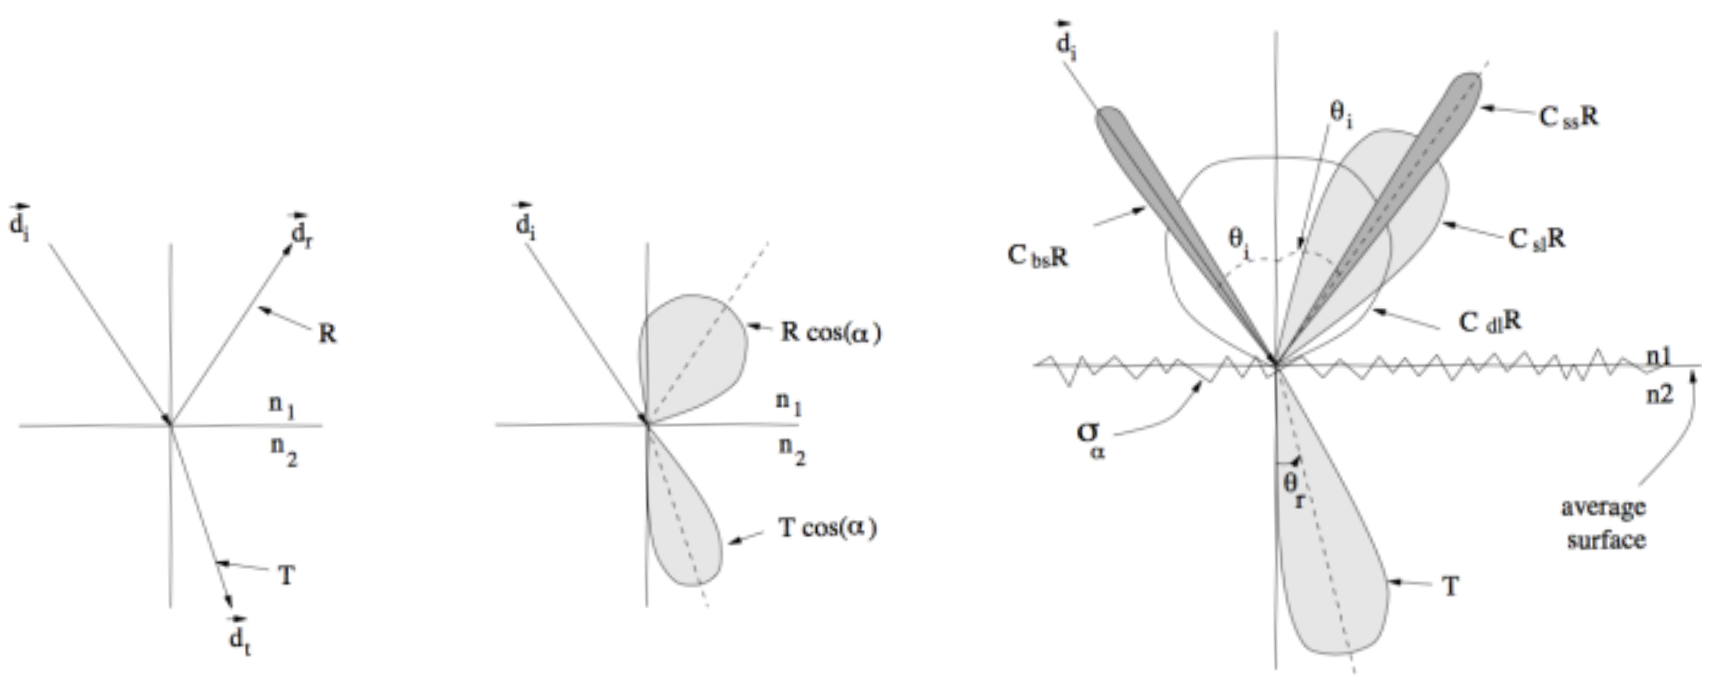
\includegraphics[width=1.0\columnwidth]{simulation/figs/polished_vs_ground_v2}
	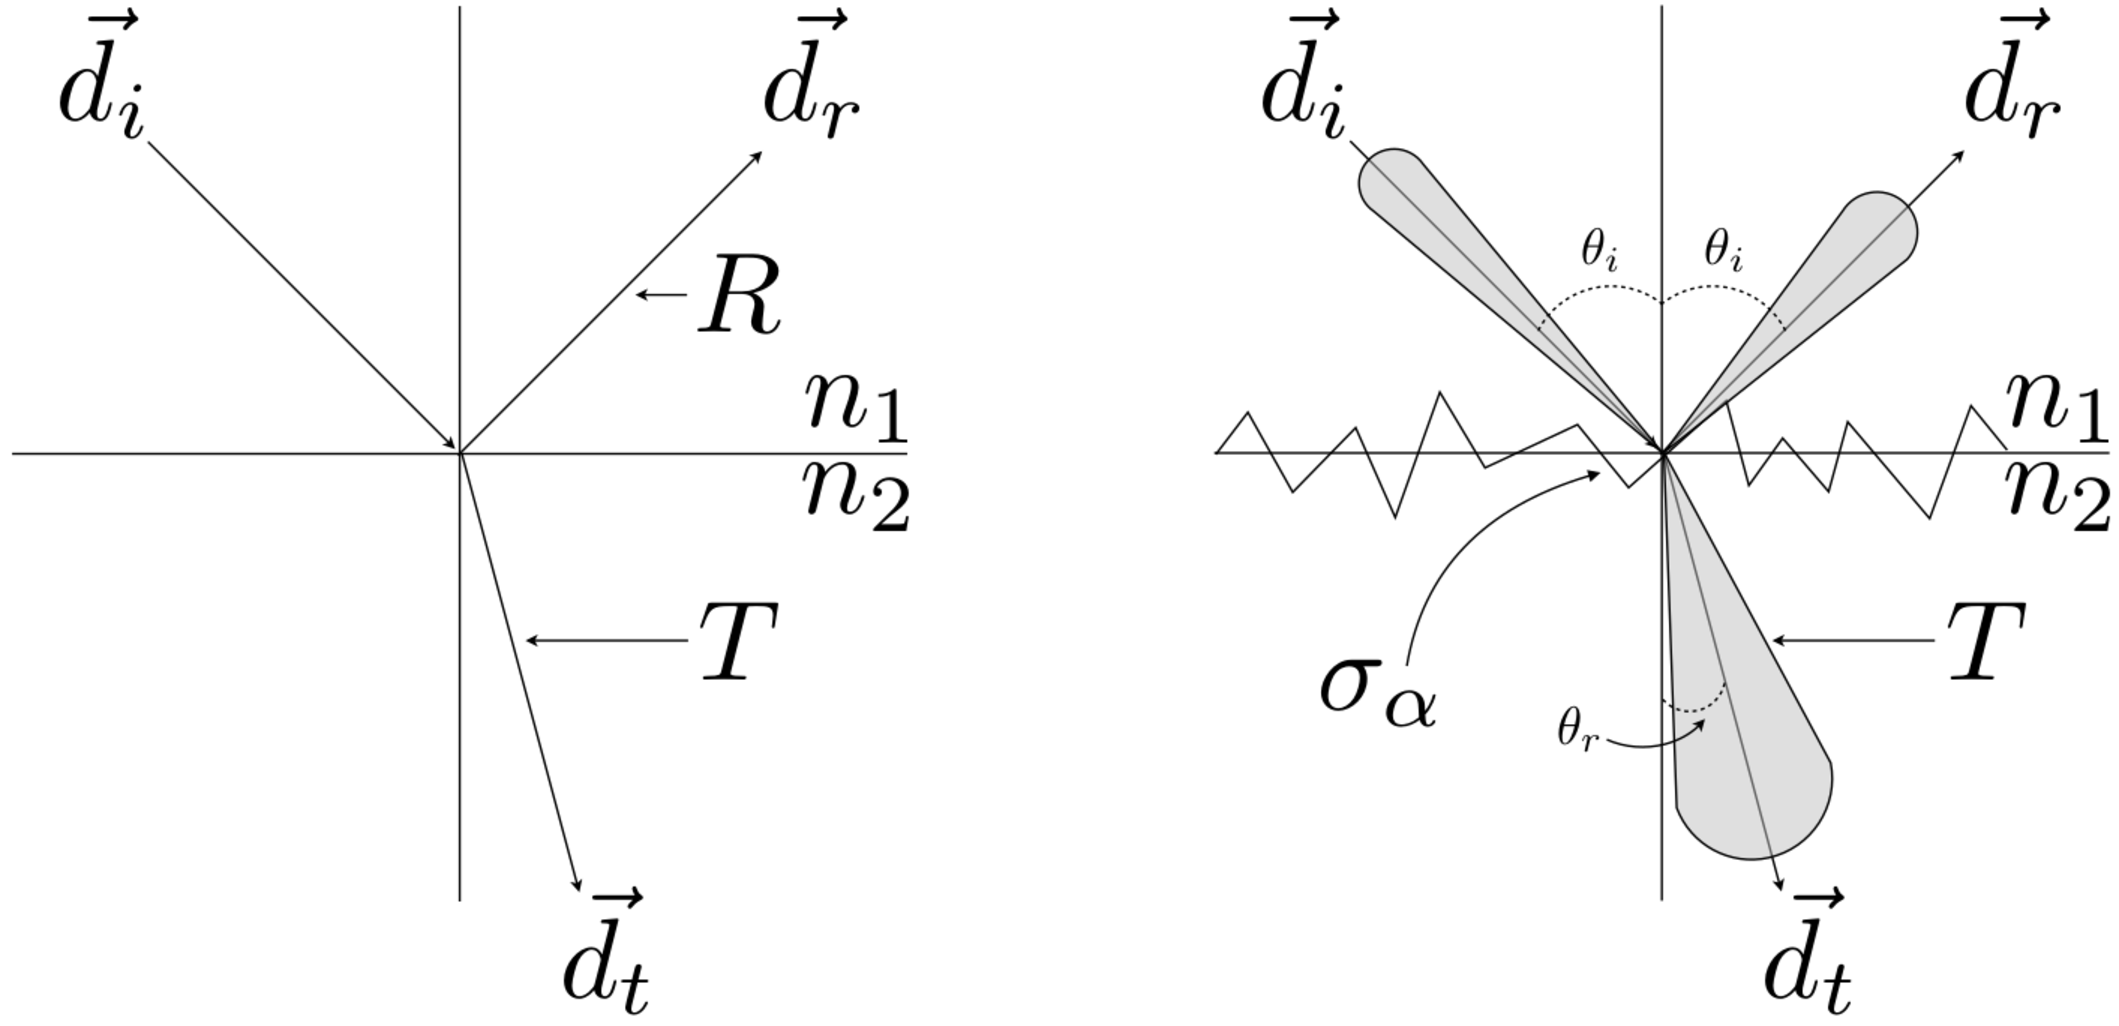
\includegraphics[width=1.0\columnwidth]{simulation/figs/st_unified_sim_v2}
	\caption{POLISH and UNIFIED models of scintillator surfaces.  Left: Polar plot of the radiant intensity of the POLISH model.  Right: Polar plot of the radiant intensity in the UNIFIED model \cite{scint_surface_sim}.}
	\label{fig:polished_vs_ground}
	\end{figure}
The details of the UNIFIED model parameters are discussed in detail in Ref.~\cite{pooser16} \& \cite{scint_surface_sim}.

%In the polished model, Fresnel reflection and refraction is assumed, where as the ground model allows for Lambertian reflection, Fresnel refraction, backscattering, as well as spike and lobe reflections.  The spike ($C_{ss}$) reflection parameter assumes the optical photons are reflected as if the surface was a perfect mirror.  The backscattering ($C_{bs}$) reflection parameter assumes the photon is reflected in the same direction of incidence.  The Lambertian ($C_{dl}$) reflection parameter assumes that the photons are reflected corresponding to a Lambertian distribution.  The lobe ($C_{sl}$) reflection parameter assumes that the photons will reflect based on the orientation of the micro-facet on the scintillator surface, where $\sigma_{\alpha}$ defines the standard deviation of the distribution of the micro-facets orientation \cite{scint_surface_sim}.  One caveat of the aforementioned models is that they assume identical parameters for the entire optical surface \cite{puneet_sim_wiki}.

As was done in section \ref{sec:sim_simple}, 10,000 optical photons were generated in the scintillator medium every 2.5 cm and the number of hits collected in the SiPM were recorded.  For the POLISH model, the transmission efficiency $\epsilon$ was varied and the attenuation length $\alpha$ was extracted for various values of $\epsilon$ in the straight region.  For the UNIFIED model, $\epsilon$ was held constant along with the radiant intensity parameters while $\sigma_{\alpha}$, which characterizes the standard deviation of the surfaces micro-facet orientation, was varied.  In a similar manner to the POLISH model, $\alpha$ was extracted in order to characterize the straight section.  The results of these simulations are show in Fig. \ref{fig:transm_eff_vs_sig_alpha}.
	\begin{figure}[!htb]
	\centering
	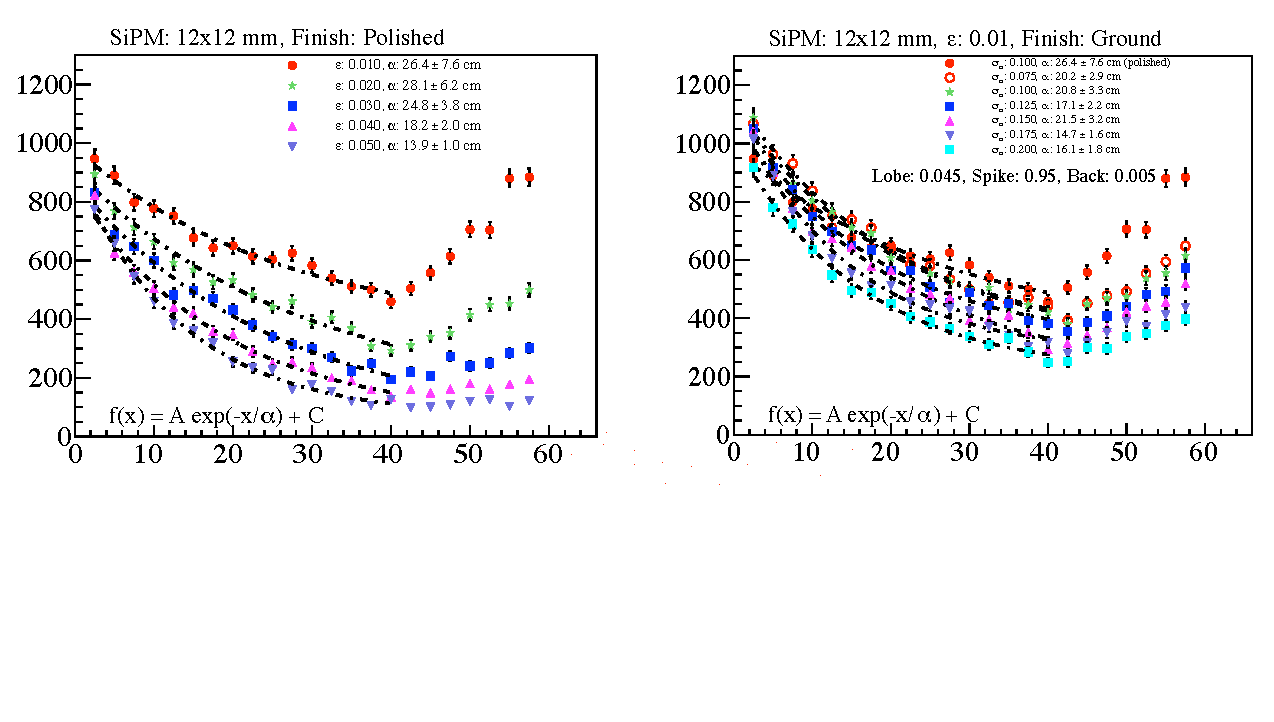
\includegraphics[width=1.0\columnwidth]{simulation/figs/transm_eff_vs_sig_alpha}
	\caption{POLISH and UNIFIED model results.  The number of hits recorded in the SiPM are plotted against the source distance (cm).  Left: POLISH model while varying the transmission efficiency $\epsilon$.  Right: UNIFIED model while varying the standard deviation of the surfaces micro-facet orientation $\sigma_{\alpha}$.}
	\label{fig:transm_eff_vs_sig_alpha}
	\end{figure}

It is clear that if the transmission efficiency is increased while assuming a perfectly polished surface, the amount of light collected in the SiPM also increases as illustrated in Fig.~\ref{fig:transm_eff_vs_sig_alpha}.  Similarly, as the number of micro-facet orientations increase, meaning a more coarsely ground surface, the amount of light collection in the SiPM decreases.  Moreover, in the instances where the surface quality of the machined scintillators are good, the phenomenon of light increase in the nose region as the source moves further from the readout detector is observed.